\paragraph{Phân tích bộ dữ liệu Telco Churn} \hfill \\
Dự báo khả năng khách hàng rời bỏ dịch vụ viễn thông. Đây là bài toán phân loại nhị phân tiêu biểu.

\paragraph{Phân tích biến mục tiêu và các yếu tố ảnh hưởng} \hfill \\
Tỷ lệ khách hàng rời bỏ (Churn) chiếm khoảng 26.5\% dữ liệu, tạo ra sự mất cân bằng nhẹ:
\begin{figure}[H]
    \centering
    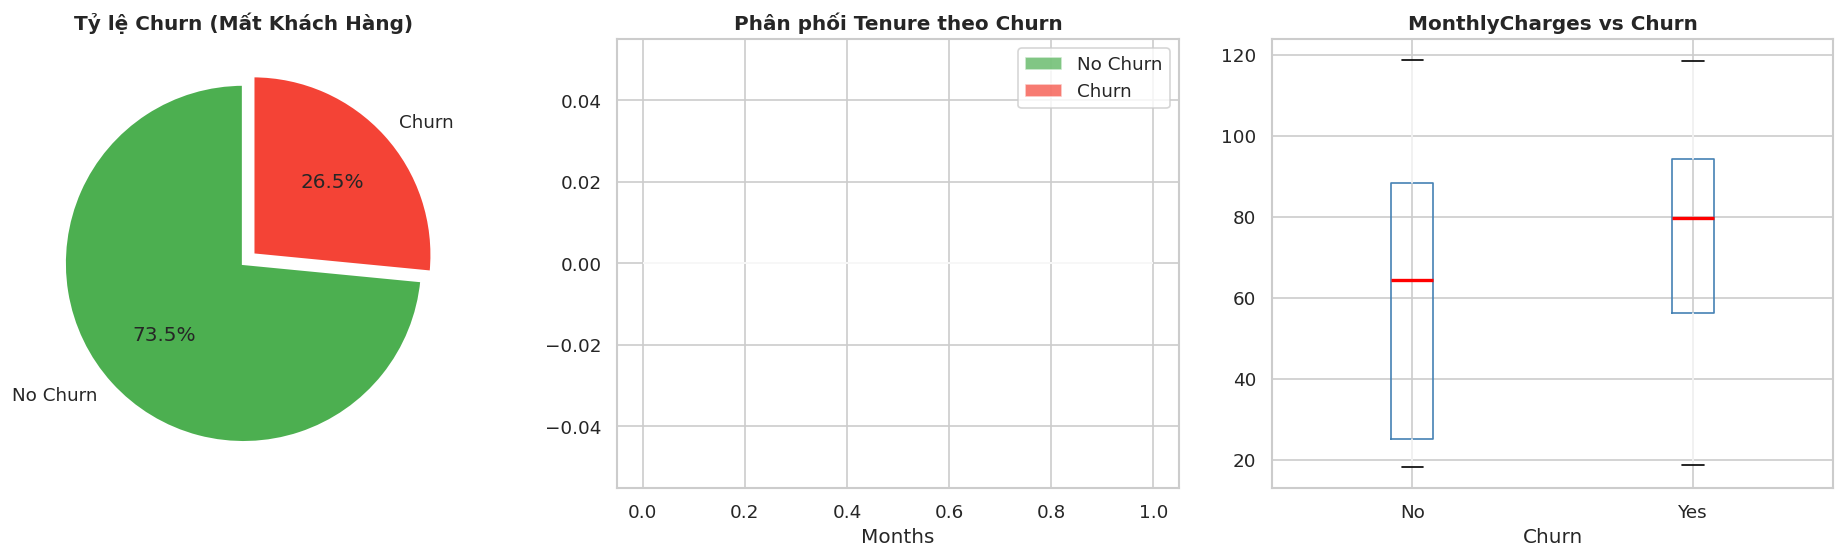
\includegraphics[width=0.8\linewidth]{Chương_1/results/telco/01_churn_eda.png}
    \caption{Phân phối nhãn Churn và thời gian gắn bó (Tenure)}
\end{figure}

Hình 1.9 cho thấy khách hàng mới (Tenure thấp) có xu hướng rời bỏ dịch vụ cao hơn hẳn khách hàng lâu năm. Điều này gợi ý rằng các chương trình khuyến mãi nên tập trung vào giai đoạn đầu của hợp đồng.

Chúng ta quan sát thấy khách hàng sử dụng hợp đồng ngắn hạn (Month-to-month) và thanh toán bằng séc điện tử (Electronic check) có tỷ lệ rời bỏ cao nhất:
\begin{figure}[H]
    \centering
    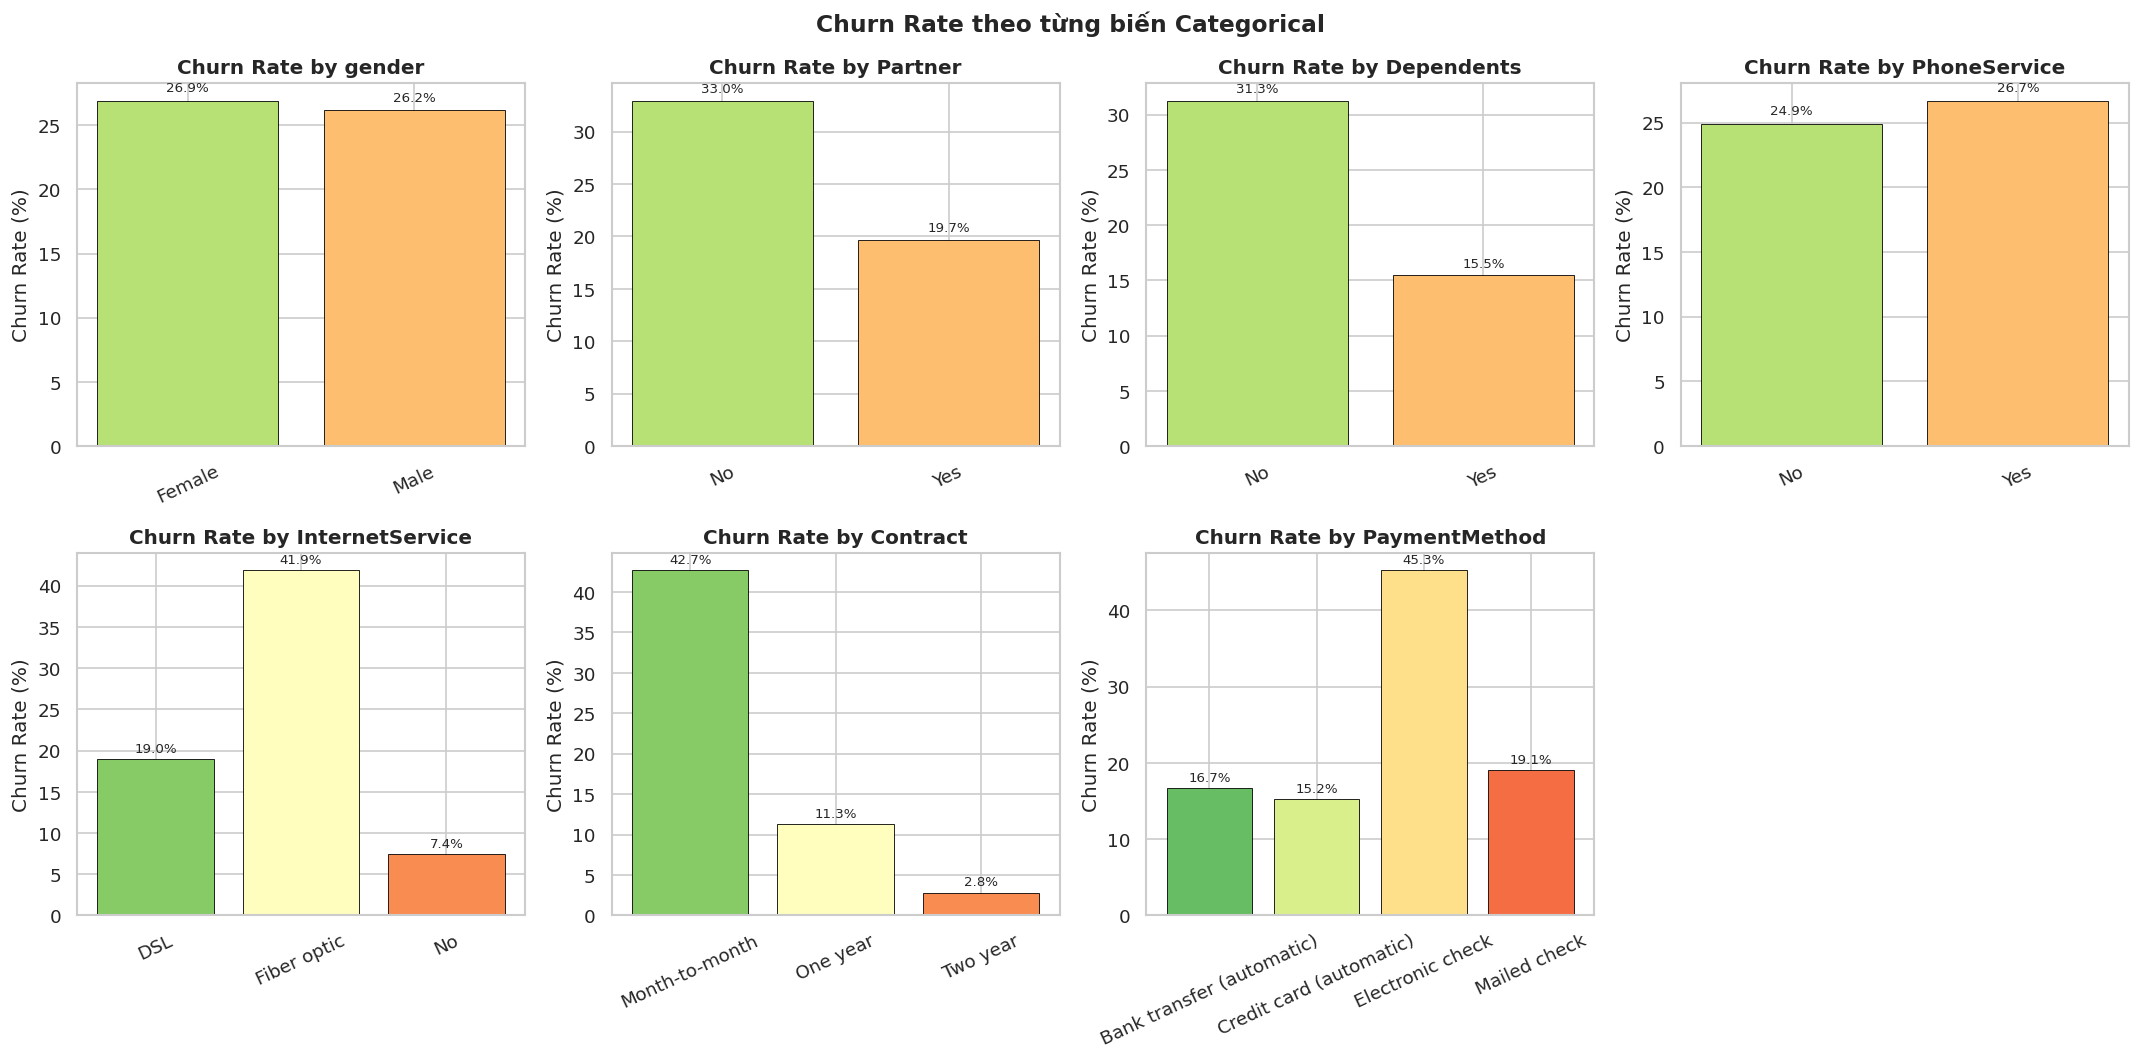
\includegraphics[width=0.8\linewidth]{Chương_1/results/telco/02_churn_by_category.png}
    \caption{Tỷ lệ rời bỏ theo loại hợp đồng và phương thức thanh toán}
\end{figure}

Hình 1.10 chỉ ra rằng loại hợp đồng là yếu tố then chốt: khách hàng "Month-to-month" có rủi ro rời bỏ cao nhất, trong khi hợp đồng 1-2 năm giúp duy trì sự ổn định. Thanh toán qua "Electronic check" cũng là một dấu hiệu cảnh báo cần chú ý.

\paragraph{Kỹ thuật xử lý: Cân bằng dữ liệu với SMOTE} \hfill \\
Để mô hình không bị thiên kiến về lớp đa số, kỹ thuật SMOTE được áp dụng để sinh thêm các mẫu giả lập cho lớp Churn:
\begin{figure}[H]
    \centering
    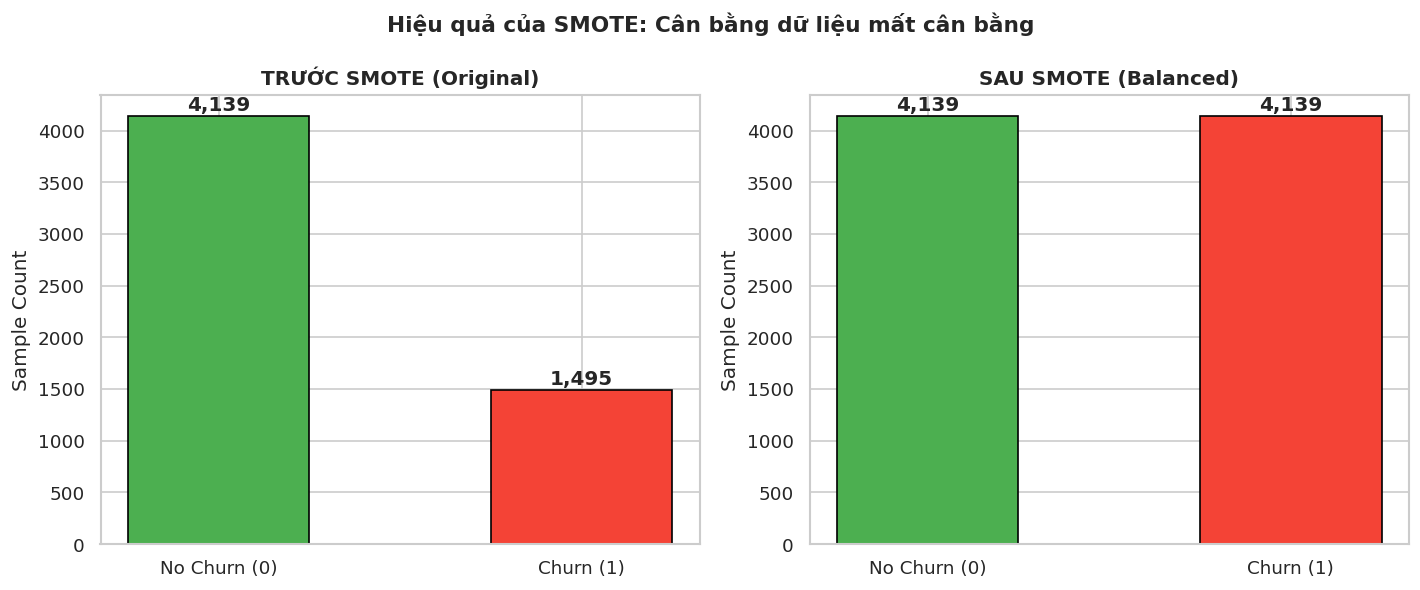
\includegraphics[width=0.8\linewidth]{Chương_1/results/telco/03_smote_comparison.png}
    \caption{Tương quan dữ liệu trước và sau khi áp dụng SMOTE}
\end{figure}

Hình 1.11 minh họa hiệu quả của kỹ thuật SMOTE. Bằng cách sinh thêm các mẫu giả lập cho lớp thiểu số dựa trên khoảng cách K-Nearest Neighbors, chúng ta đã cân bằng được tập huấn luyện, giúp mô hình học được đặc trưng của nhóm khách hàng rời bỏ một cách công bằng hơn.

\paragraph{Kết quả thực nghiệm} \hfill \\
Thực nghiệm sử dụng Logistic Regression và Random Forest với bộ tham số cân bằng.

\begin{table}[H]
    \centering
    \begin{tabular}{|l|c|c|c|c|}
    \hline
    \textbf{Mô hình} & \textbf{Accuracy} & \textbf{ROC-AUC} & \textbf{F1 (Churn)} & \textbf{Recall (Churn)} \\ \hline
    Logistic Regression & 0.7949 & 0.8407 & 0.61 & 0.61 \\ \hline
    Random Forest & 0.7786 & 0.8197 & 0.57 & 0.55 \\ \hline
    \end{tabular}
    \caption{Kết quả phân loại khách hàng rời bỏ}
\end{table}

\begin{figure}[H]
    \centering
    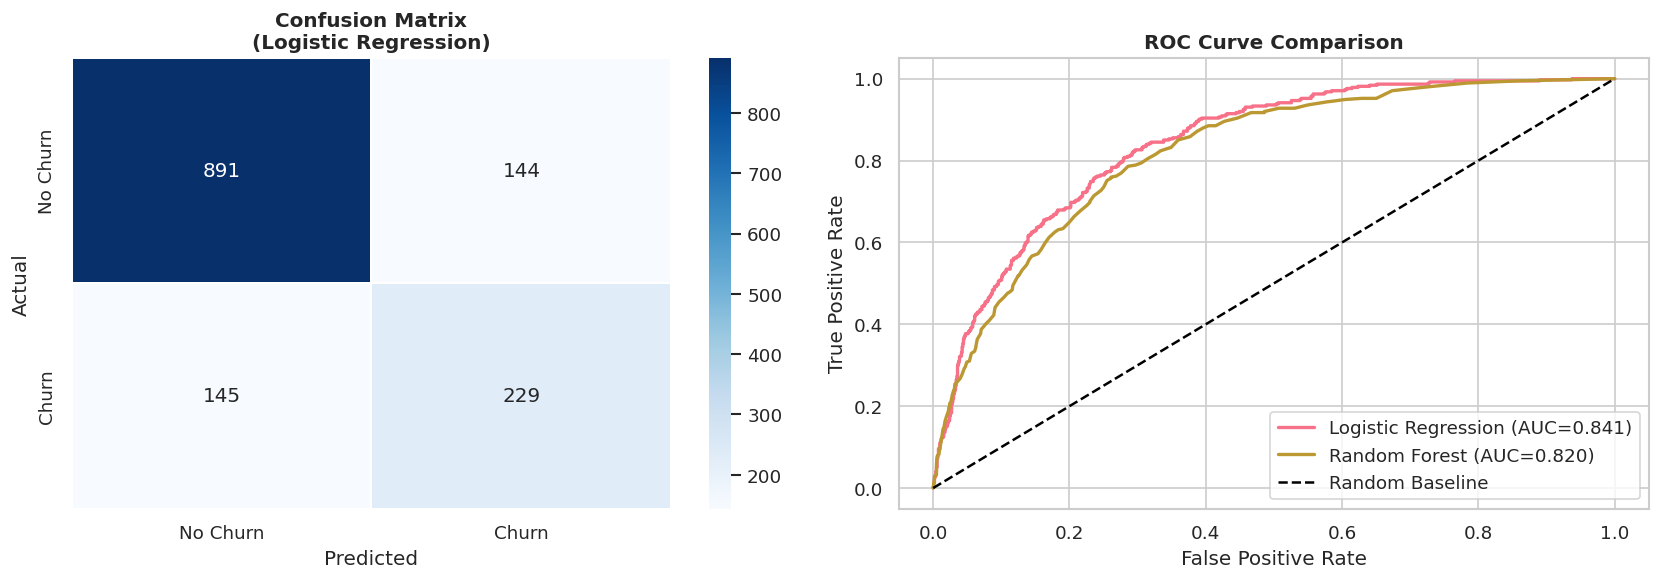
\includegraphics[width=0.8\linewidth]{Chương_1/results/telco/04_confusion_roc.png}
    \caption{Ma trận nhầm lẫn và Đường cong ROC (Logistic Regression chiếm ưu thế)}
\end{figure}

Hình 1.12 cho thấy mô hình Logistic Regression đạt diện tích dưới đường cong (AUC) là 0.84, một con số khá tốt cho bài toán dự báo hành vi con người. Ma trận nhầm lẫn xác nhận khả năng cân bằng giữa việc phát hiện Churn và duy trì độ chính xác tổng thể.

\paragraph{Feature Importance} \hfill \\
Biểu đồ dưới đây chỉ ra các yếu tố "giữ chân" khách hàng hiệu quả nhất:
\begin{figure}[H]
    \centering
    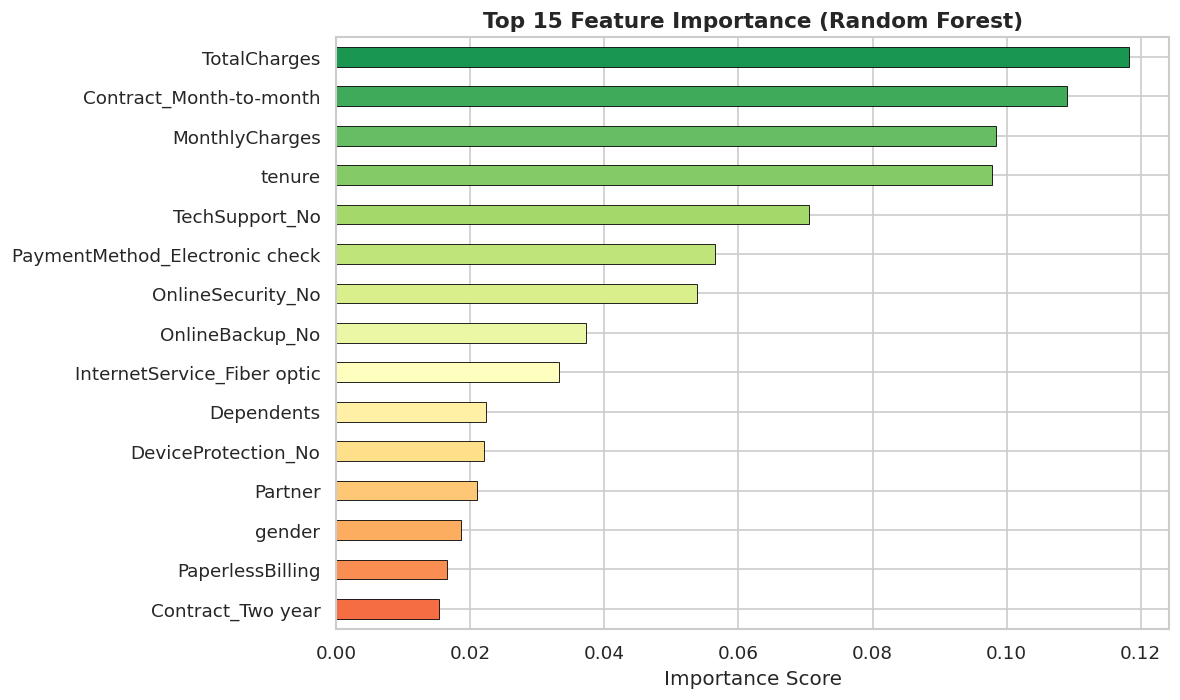
\includegraphics[width=0.8\linewidth]{Chương_1/results/telco/05_feature_importance.png}
    \caption{Tầm quan trọng của các đặc trưng trong bài toán Churn}
\end{figure}

Hình 1.13 tổng kết các đặc trưng quan trọng nhất. Ngoài loại hợp đồng và thời gian gắn bó, tổng số tiền thanh toán (\texttt{TotalCharges}) và loại hình Internet cũng đóng vai trò quyết định trong việc dự báo khả năng khách hàng rời đi.

\paragraph{Phụ lục: Chi tiết quá trình thực hiện thực nghiệm Telco Churn} \hfill \\
Dưới đây là các bước thực hiện chi tiết cho bài toán dự báo khách hàng rời bỏ dịch vụ.

\begin{figure}[H]
    \centering
    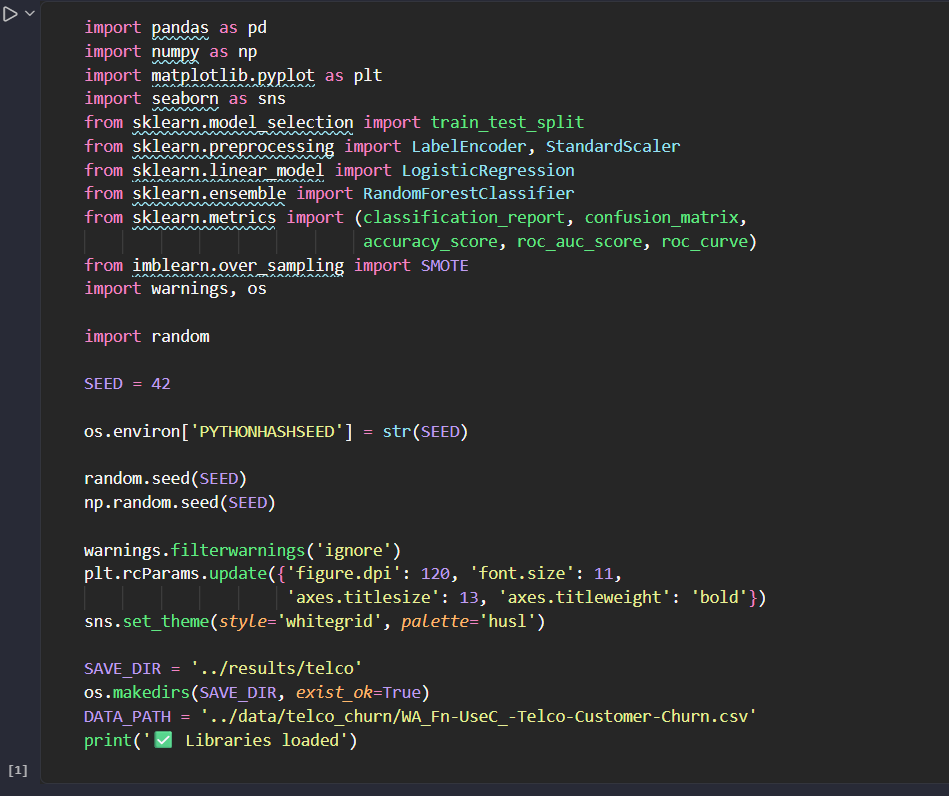
\includegraphics[width=0.9\linewidth]{Chương_1/docs/ch1/28.png}
    \caption{Khởi tạo: Import các thư viện xử lý dữ liệu và học máy cho bài toán phân loại.}
\end{figure}

\begin{figure}[H]
    \centering
    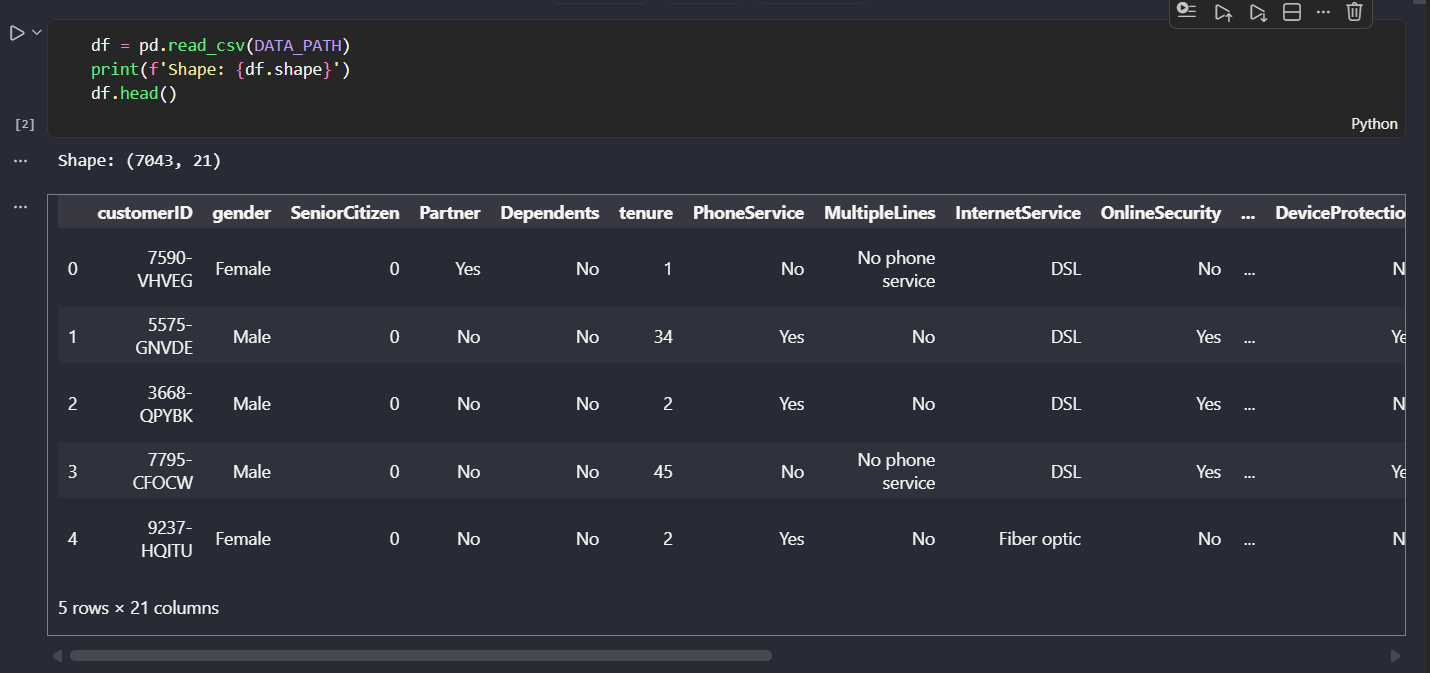
\includegraphics[width=0.9\linewidth]{Chương_1/docs/ch1/29.png}
    \caption{Tải dữ liệu Telco Churn: Đọc dữ liệu và kiểm tra phân phối của biến mục tiêu Churn.}
\end{figure}

\begin{figure}[H]
    \centering
    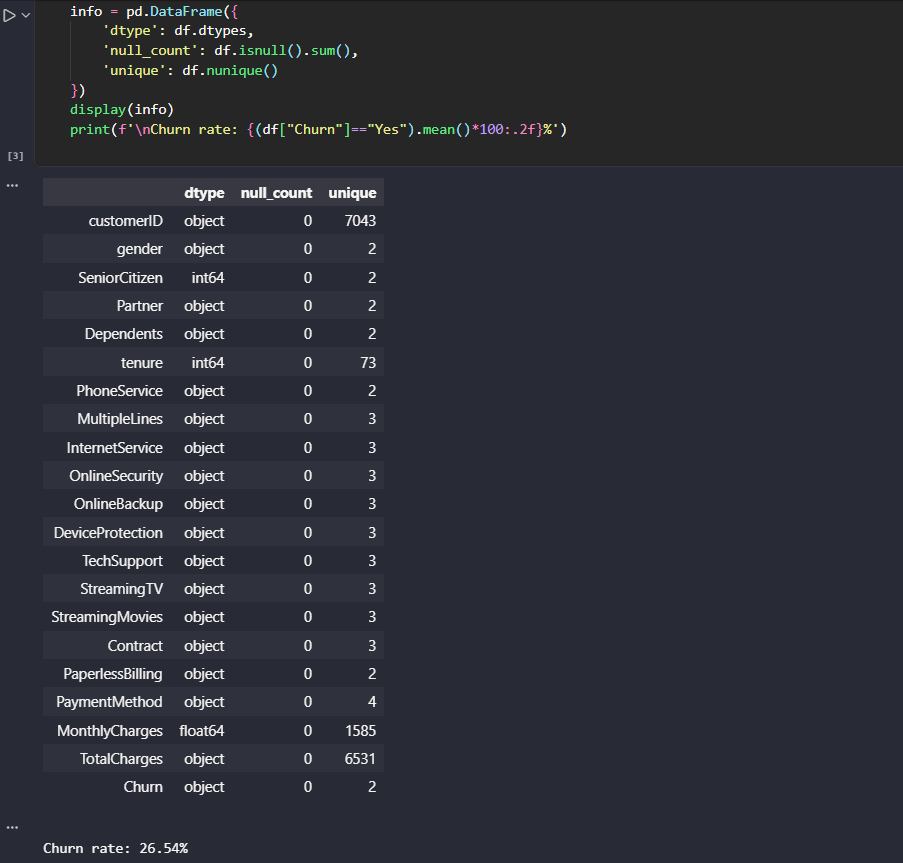
\includegraphics[width=0.9\linewidth]{Chương_1/docs/ch1/30.png}
    \caption{Thống kê cơ bản: Xem xét kiểu dữ liệu và tỷ lệ khách hàng rời bỏ (26.54\%).}
\end{figure}

\begin{figure}[H]
    \centering
    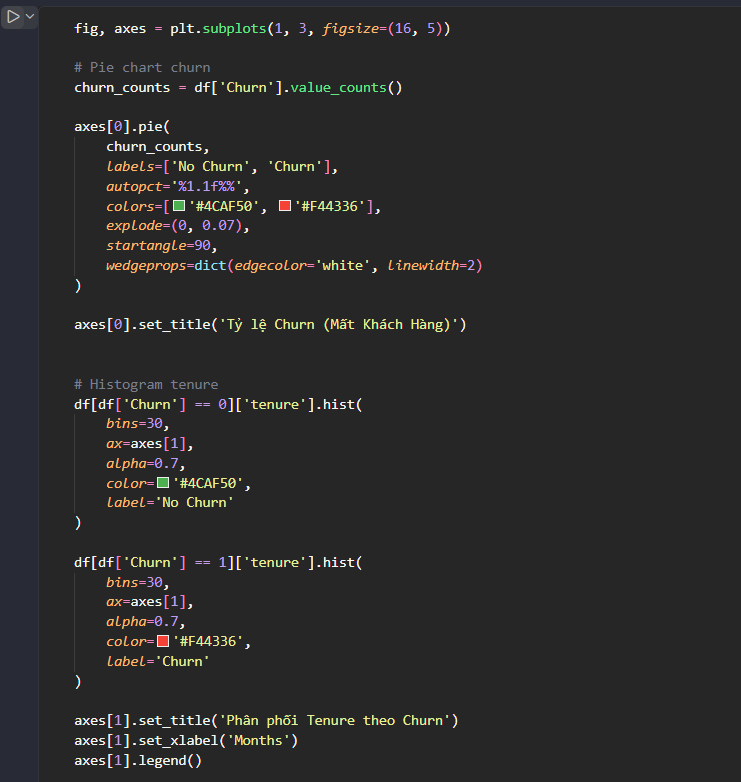
\includegraphics[width=0.9\linewidth]{Chương_1/docs/ch1/31.png}
    \caption{Mã nguồn EDA (Phần 1): Vẽ biểu đồ tròn tỷ lệ Churn và biểu đồ histogram cho Tenure.}
\end{figure}

\begin{figure}[H]
    \centering
    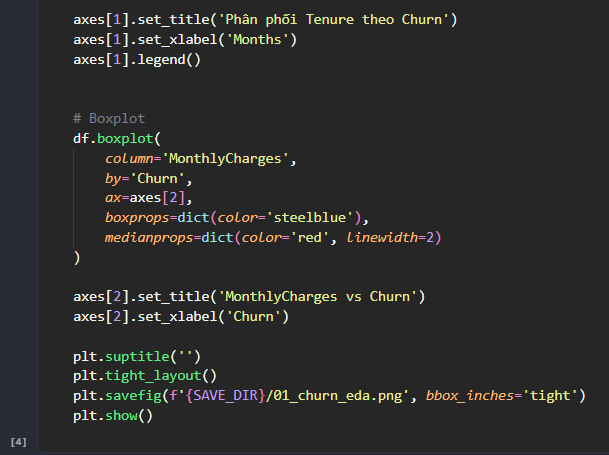
\includegraphics[width=0.9\linewidth]{Chương_1/docs/ch1/32.png}
    \caption{Mã nguồn EDA (Phần 2): Bổ sung biểu đồ Boxplot cho chi phí hàng tháng (Monthly Charges).}
\end{figure}

\begin{figure}[H]
    \centering
    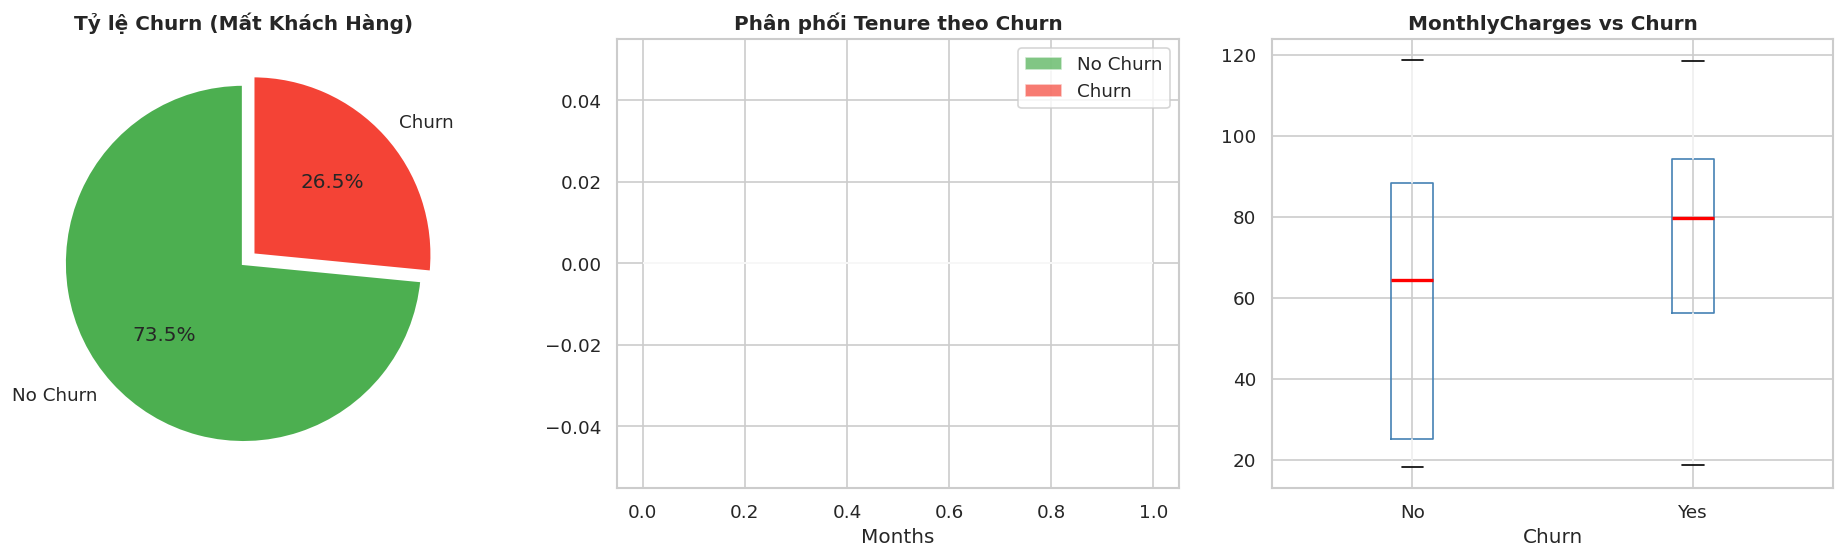
\includegraphics[width=0.9\linewidth]{Chương_1/docs/ch1/33.png}
    \caption{Kết quả EDA tổng quan: Nhận diện sự khác biệt về Tenure và Chi phí giữa hai nhóm khách hàng.}
\end{figure}

\begin{figure}[H]
    \centering
    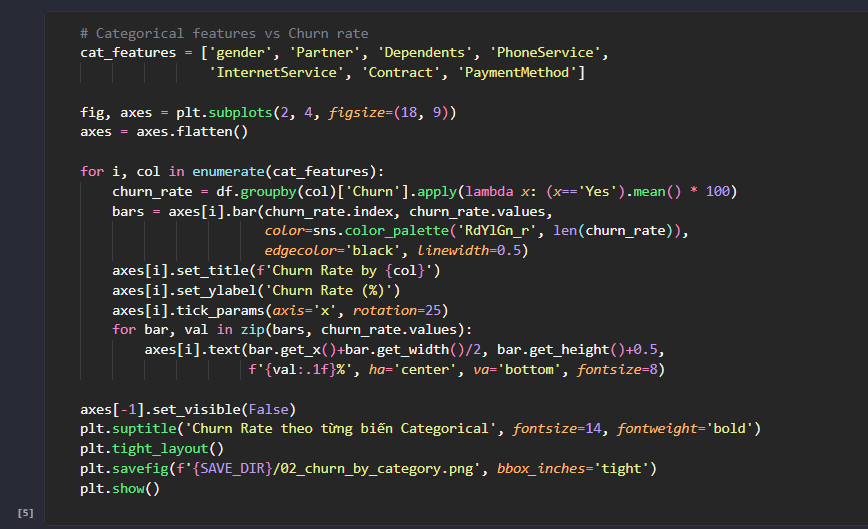
\includegraphics[width=0.9\linewidth]{Chương_1/docs/ch1/34.png}
    \caption{Mã nguồn phân tích biến hạng mục: So sánh tỷ lệ Churn theo các loại dịch vụ và hợp đồng.}
\end{figure}

\begin{figure}[H]
    \centering
    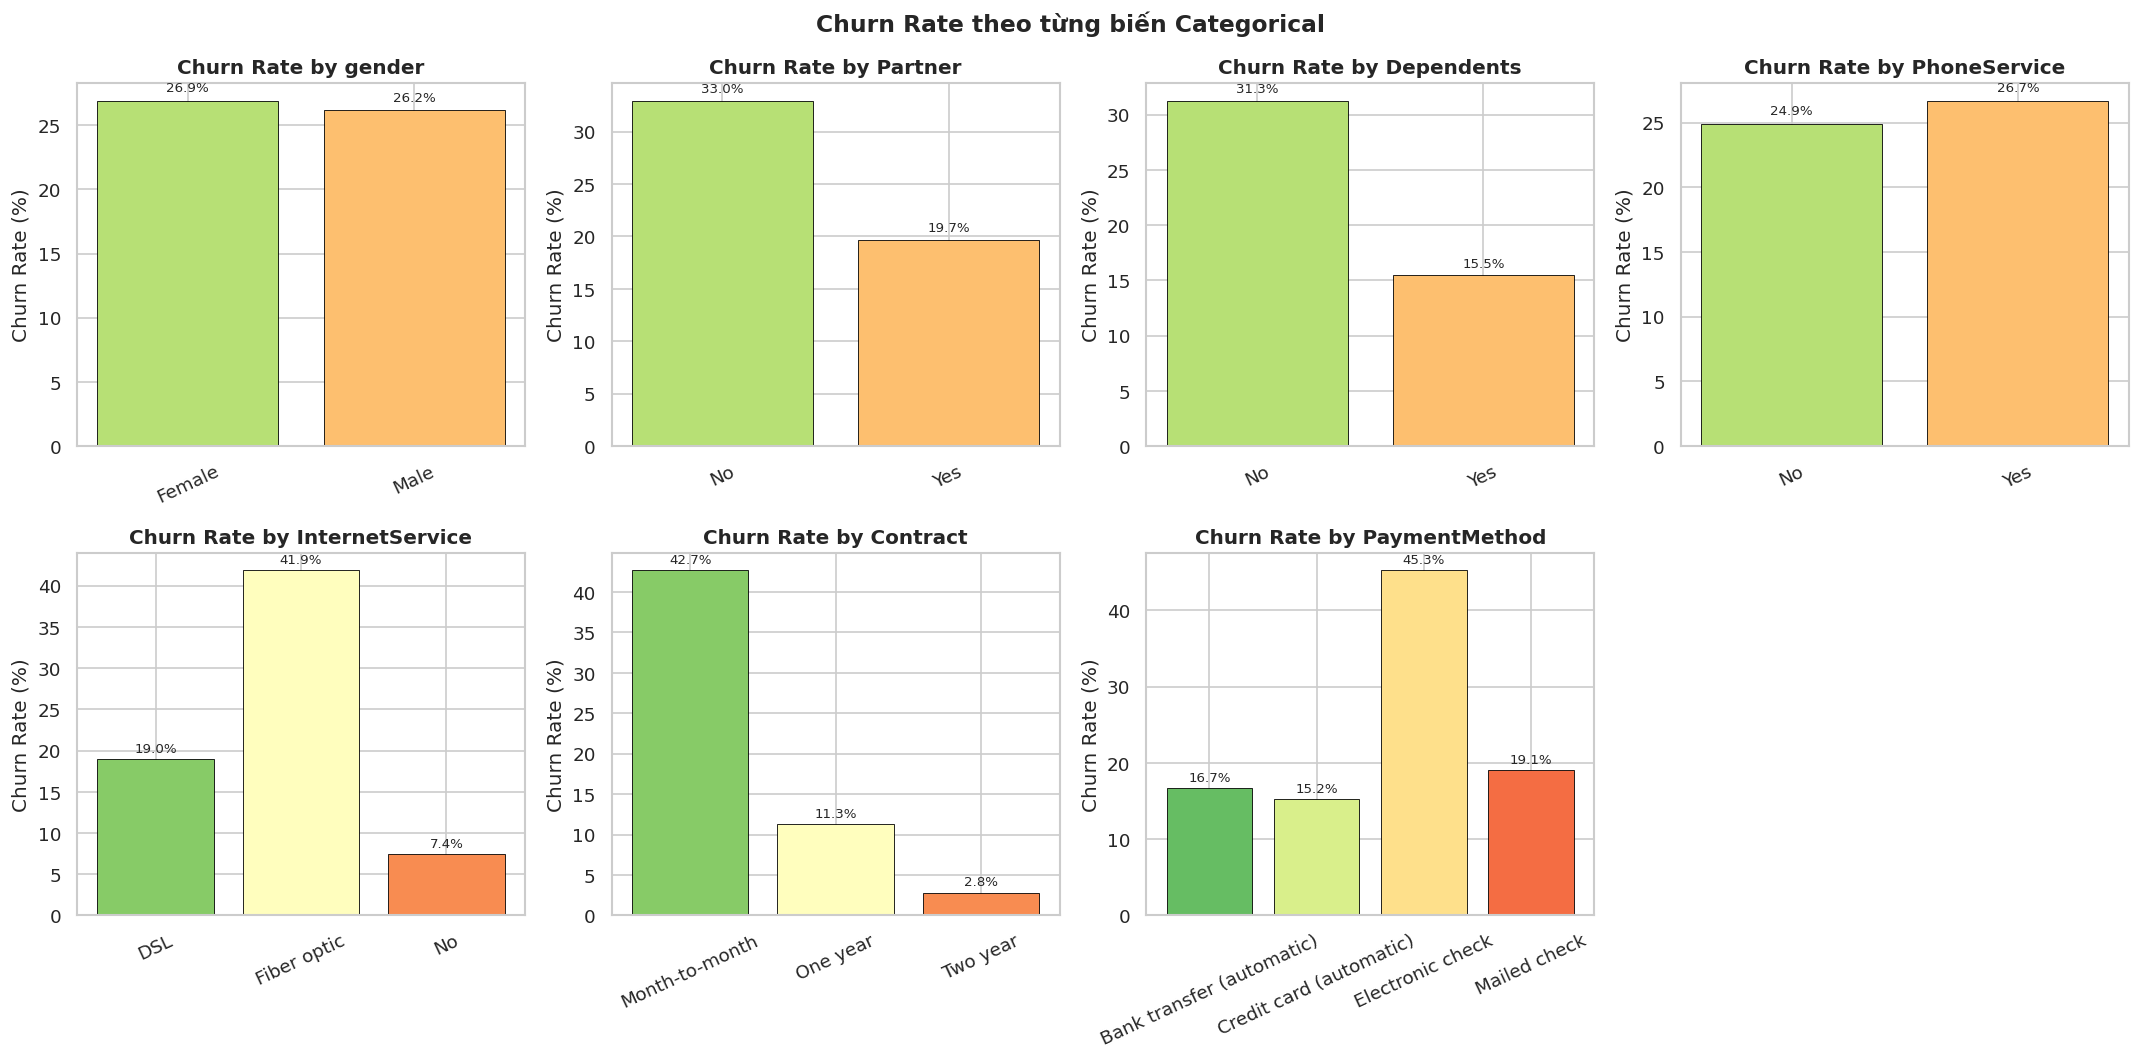
\includegraphics[width=0.9\linewidth]{Chương_1/docs/ch1/35.png}
    \caption{Kết quả phân tích hạng mục: Khách hàng dùng hợp đồng Month-to-month có tỷ lệ rời đi cao nhất.}
\end{figure}

\begin{figure}[H]
    \centering
    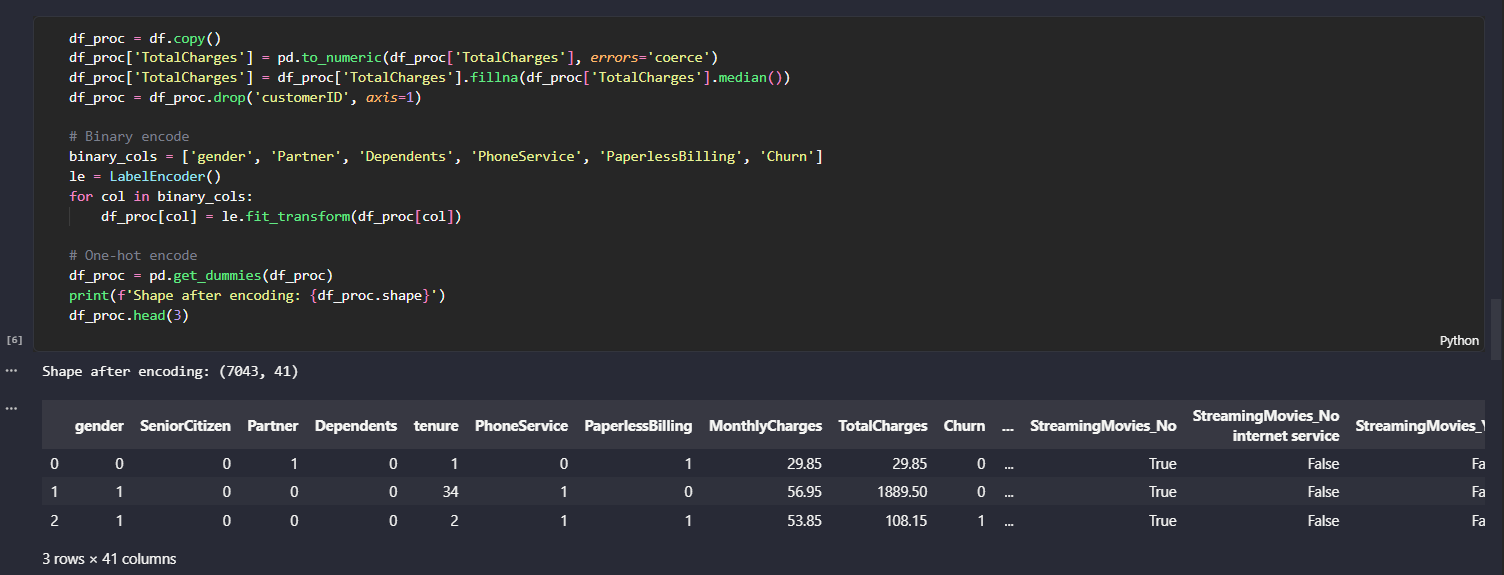
\includegraphics[width=0.9\linewidth]{Chương_1/docs/ch1/36.png}
    \caption{Mã nguồn Heatmap tương quan: Đánh giá mối liên hệ giữa các biến số sau khi mã hóa.}
\end{figure}

\begin{figure}[H]
    \centering
    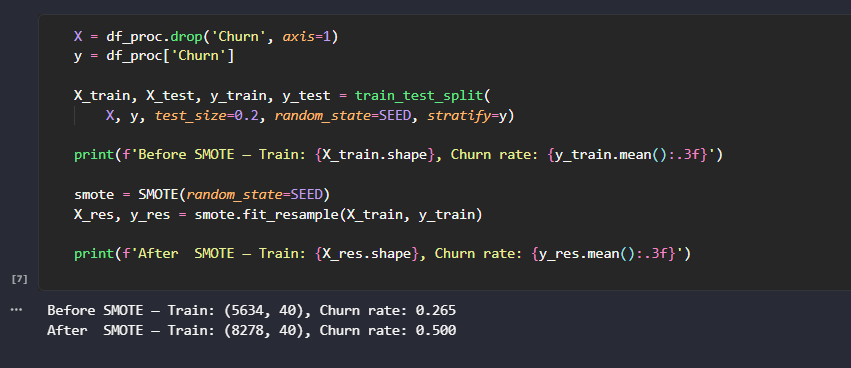
\includegraphics[width=0.9\linewidth]{Chương_1/docs/ch1/37.png}
    \caption{Kết quả Ma trận tương quan: Quan sát các biến có tương quan thuận/nghịch với Churn.}
\end{figure}

\begin{figure}[H]
    \centering
    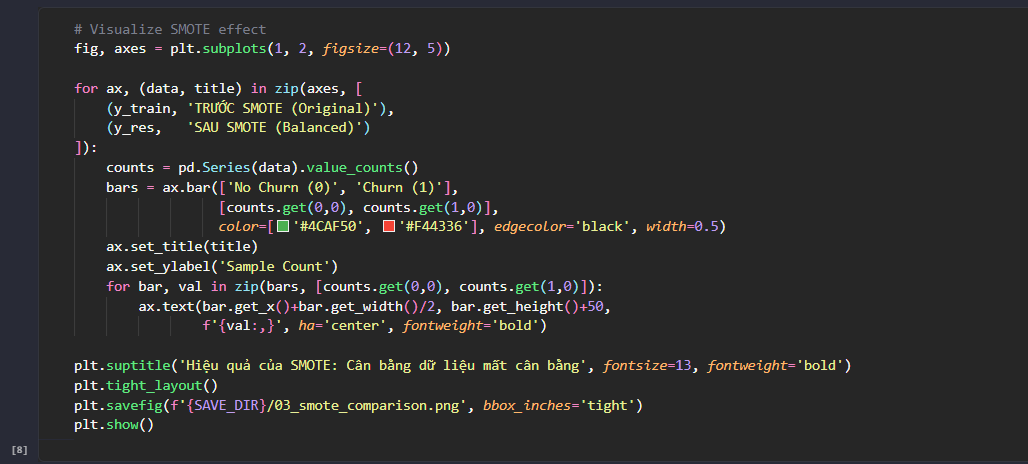
\includegraphics[width=0.9\linewidth]{Chương_1/docs/ch1/38.png}
    \caption{Tiền xử lý và SMOTE: Mã nguồn xử lý giá trị thiếu, mã hóa Label/One-hot và cân bằng dữ liệu.}
\end{figure}

\begin{figure}[H]
    \centering
    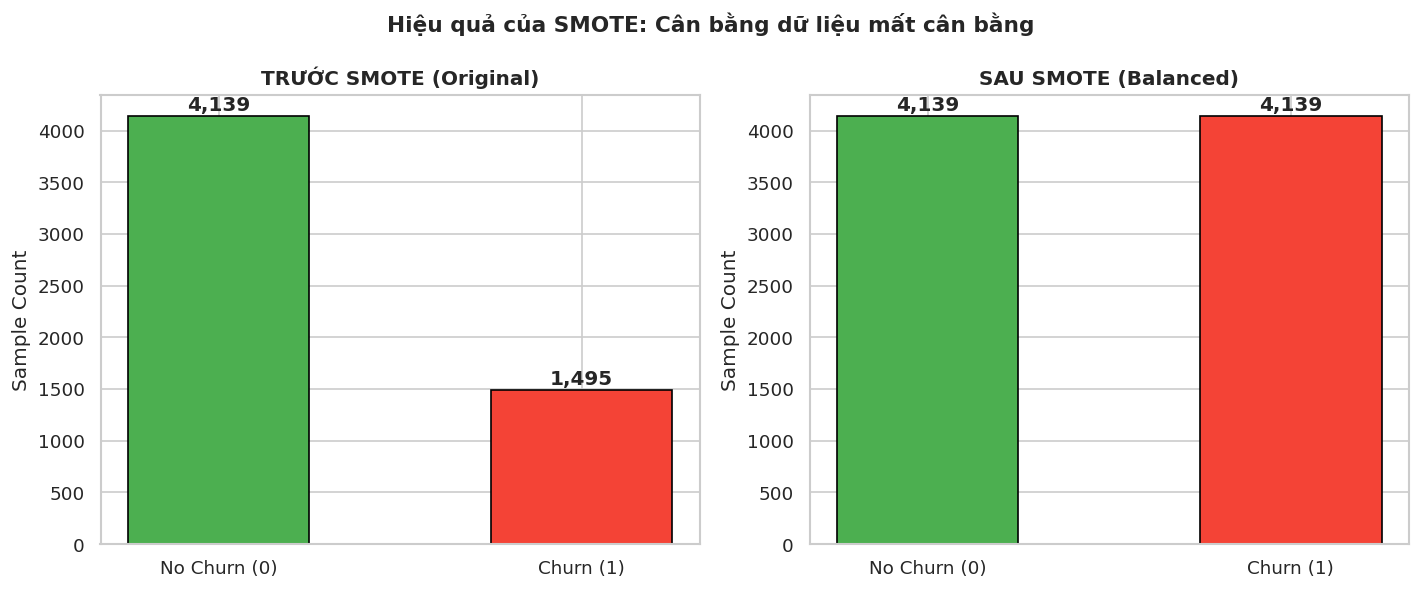
\includegraphics[width=0.9\linewidth]{Chương_1/docs/ch1/39.png}
    \caption{Kết quả SMOTE: Trực quan hóa sự thay đổi phân phối dữ liệu trước và sau khi Over-sampling.}
\end{figure}

\begin{figure}[H]
    \centering
    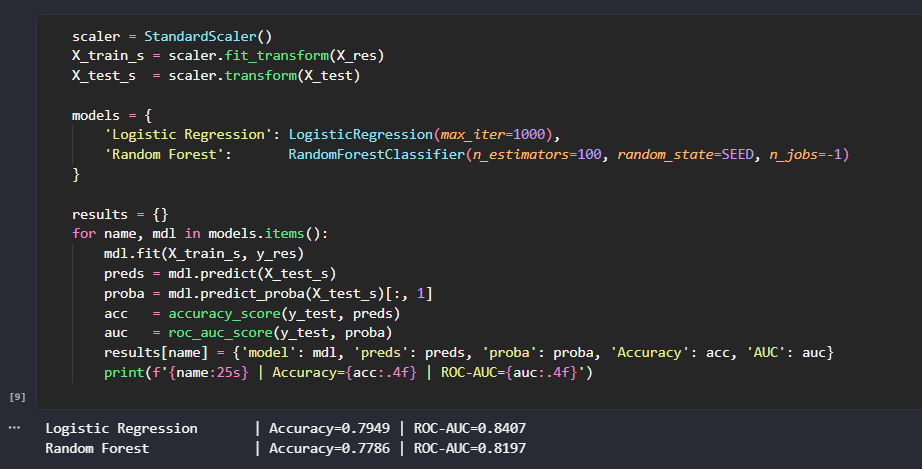
\includegraphics[width=0.9\linewidth]{Chương_1/docs/ch1/40.png}
    \caption{Huấn luyện mô hình: So sánh hiệu năng giữa Logistic Regression và Random Forest trên tập Test.}
\end{figure}

\begin{figure}[H]
    \centering
    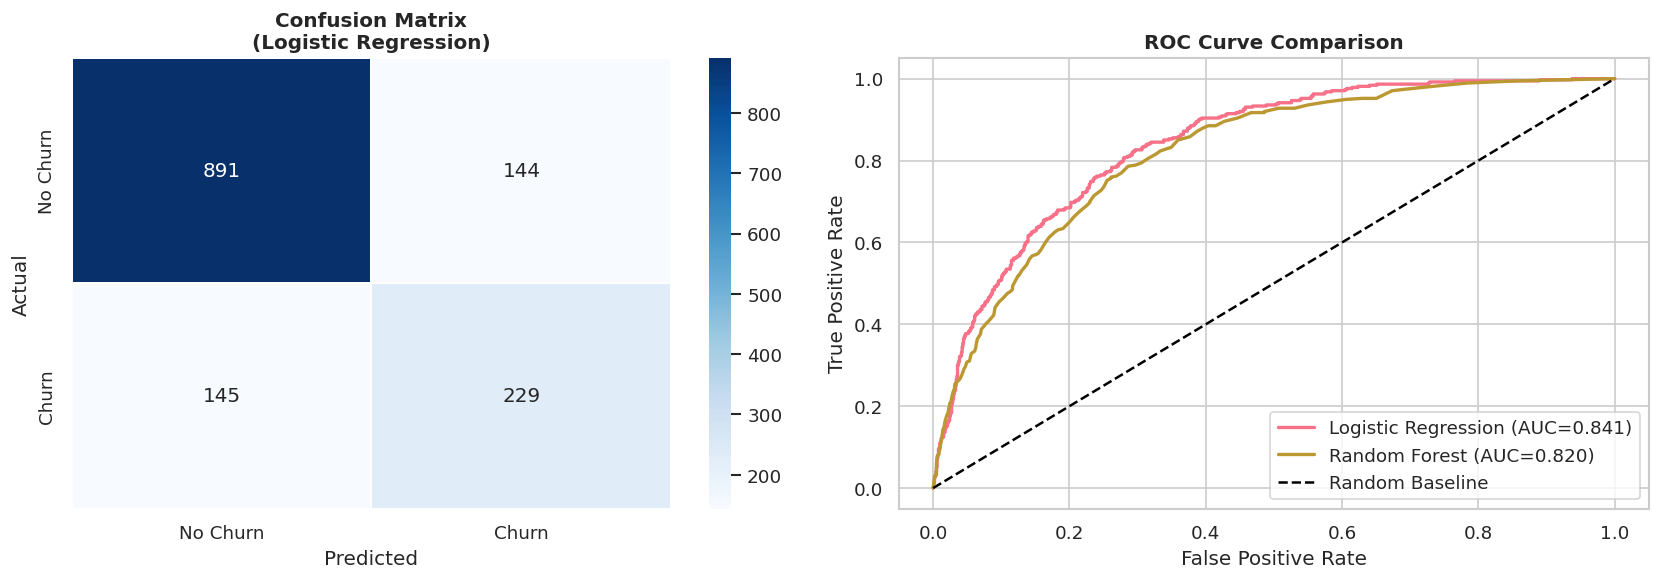
\includegraphics[width=0.9\linewidth]{Chương_1/docs/ch1/41.png}
    \caption{Mã nguồn đánh giá chi tiết: Vẽ Ma trận nhầm lẫn và đường cong ROC cho các mô hình.}
\end{figure}

\begin{figure}[H]
    \centering
    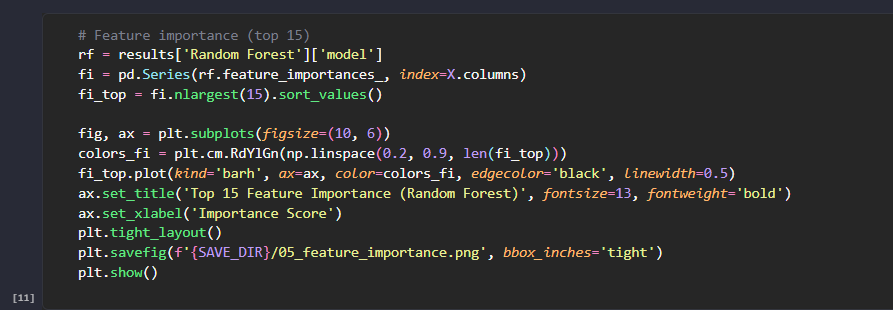
\includegraphics[width=0.9\linewidth]{Chương_1/docs/ch1/42.png}
    \caption{Kết quả đánh giá: Logistic Regression cho thấy kết quả ổn định hơn với AUC đạt 0.84.}
\end{figure}

\begin{figure}[H]
    \centering
    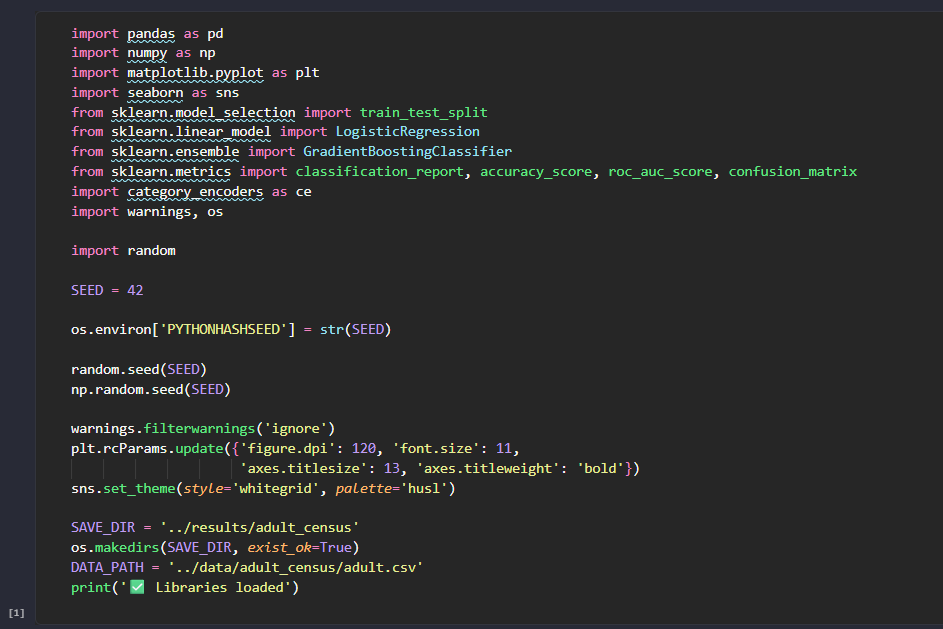
\includegraphics[width=0.9\linewidth]{Chương_1/docs/ch1/43.png}
    \caption{Tầm quan trọng của đặc trưng: Xác định các yếu tố then chốt dẫn tới quyết định rời mạng của khách hàng.}
\end{figure}
    
